\documentclass[12pt]{article}

\usepackage[english, russian]{babel}
\usepackage[T2A]{fontenc}
\usepackage[utf8]{inputenc}
\usepackage[left=2cm,right=2cm, top=1cm,bottom=1.5cm,bindingoffset=0cm]{geometry}
\usepackage[explicit]{titlesec}
\usepackage{amsmath}
\usepackage{multirow}
\usepackage{bookmark}
\usepackage{minted}
\usepackage{hyperref}

\usepackage{graphicx}
\graphicspath{{images/}}
\DeclareGraphicsExtensions{.pdf,.png,.jpg}



\newcommand{\eref}[1]{\hyperref[{e:#1}]{\nameref*{e:#1} \ref*{e:#1}}}


\begin{document}
    \pagestyle{empty}
    \begin{center}
        \textbf{Федеральное государственное автономное образовательное учреждение высшего образования}

        \vspace{5pt}

        {\small
        \textbf{САНКТ-ПЕТЕРБУРГСКИЙ НАЦИОНАЛЬНЫЙ}

        \textbf{ИССЛЕДОВАТЕЛЬСКИЙ УНИВЕРСИТЕТ ИТМО}

        \textbf{ФАКУЛЬТЕТ ПРОГРАММНОЙ ИНЖЕНЕРИИ И КОМПЬЮТЕРНОЙ ТЕХНИКИ}%
        }

        \vspace{140pt}

        {\Large
        \textbf{ЗАДАНИЕ}

        \vspace{7pt}

        \textbf{ПО ДИСЦИПЛИНЕ}%
        }

        \vspace{10pt}

        {\large
        \textbf{Правовые основы интеллектуальной собственности}

        \vspace{5pt}

        \textbf{«Расчёт пошлины изобретения»}%
        }

        \vspace{170pt}

        \begin{tabular}{lll}
            Проверил:                                                                                   & \hspace{70pt} & Выполнил:                                             \\
            ........................                \rule[0.66\baselineskip]{2cm}{0.4pt}                &               & Студент группы P3555                                  \\
            «\rule[0.66\baselineskip]{1cm}{0.4pt}»  \rule[0.66\baselineskip]{2cm}{0.4pt} \the\year г.   &               & Федюкович С. А. \rule[0.66\baselineskip]{2cm}{0.4pt}  \\
            &               &                                                       \\
            Оценка          \hspace{12pt}           \rule[0.66\baselineskip]{2.7cm}{0.4pt}              &               &                                                       \\
        \end{tabular}

        \vspace*{\fill}

        Санкт-Петербург

        \the\year
    \end{center}
    \newpage
    \pagestyle{plain}
    \setcounter{page}{1}

    \section*{Задание}

    \subsection*{Условие}

    Рассчитать стоимость пошлины изобретения с формулой, состоящей из 4-ёх пунктов.

    \subsection*{Решение}

    Откроем таблицу (\href{https://rospatent.gov.ru/ru/activities/dues/table}{https://rospatent.gov.ru/ru/activities/dues/table}) видов юридически значимых действий и размеров пошлин.

    Составим сумму размера пошлины по пунктам:

    $$ 3300 (\text{пункт таблицы 1.1}) + 700 \cdot 2 (\text{пункт таблицы 1.4}) = 4700 (\text{рублей)} $$

    Сравним результат со значением калькулятора сайта Роспатента от 20 июля 2021 года:
    \begin{figure}[ht]
        \centering
        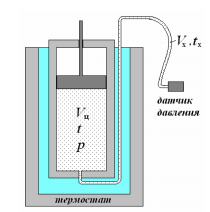
\includegraphics[scale=1.5]{images/1.png}
        \caption{Расчёт пошлины на сайте Роспатента}
        \label{fig:o:3}
    \end{figure}

    \newpage

    Аналогично получим сумму, только через калькулятор с сайта патентного бюро, например \href{https://www.vko-intellekt.ru/services/patentovanie-calculator/}{https://www.vko-intellekt.ru/services/patentovanie-calculator/}:
    \begin{figure}[ht]
        \centering
        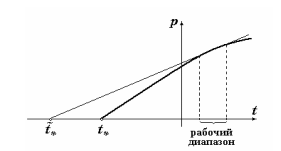
\includegraphics[scale=1.5]{images/2.png}
        \caption{Расчёт пошлины на сайте патентного бюро}
        \label{fig:o:3}
    \end{figure}


\end{document}